\lstinputlisting[float,caption={Naive kernel.}, label={naive_kernel}, 
                style=customc]{/Users/clalanne/GitHubProjects/OpenCLNotes/src/code/naive.c}

\lstinputlisting[float,caption={Kernel with more work per \emph{work item}.},label={more_work_kernel}, 
                style=customc]{/Users/clalanne/GitHubProjects/OpenCLNotes/src/code/more_work.c}

\lstinputlisting[float,caption={Kernel making use of \emph{private memory}.},label={private_memory_kernel}, 
                style=customc]{/Users/clalanne/GitHubProjects/OpenCLNotes/src/code/private_memory.c}

\lstinputlisting[float,caption={Kernel making use of \emph{private memory} and \emph{local memory}.},label={private_local_memory_kernel}, 
                style=customc]{/Users/clalanne/GitHubProjects/OpenCLNotes/src/code/private_local_memory.c}

\lstinputlisting[float,caption={Blocking \emph{kernel}.},label={tiling}, 
                style=customc]{/Users/clalanne/GitHubProjects/OpenCLNotes/src/code/block.c}

\begin{figure}[!h]
    \centering
    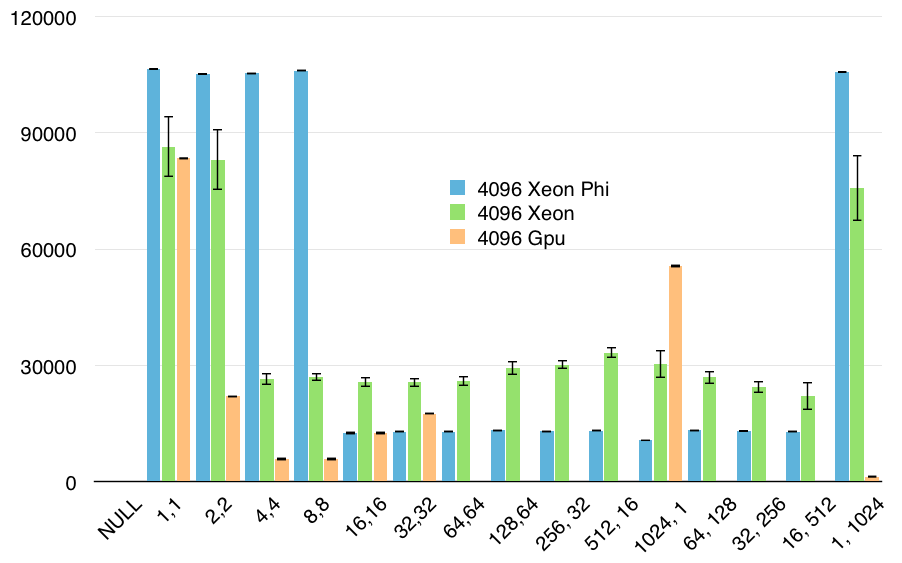
\includegraphics[width=0.6\textwidth]{figures/naive_comp.png}
    \caption{Naive matrix multiplication in different architectures comparison.}
    \label{NaiveComp}
\end{figure}

\begin{figure}[!h]
    \centering
    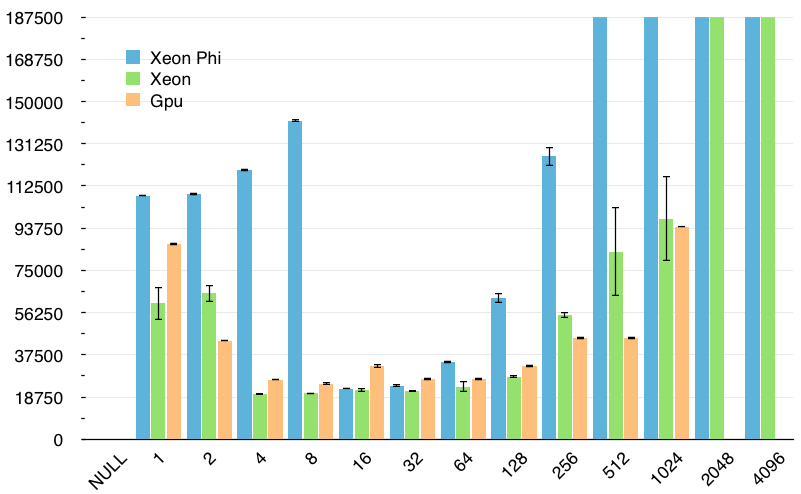
\includegraphics[width=0.6\textwidth]{figures/opt1_comp.png}
    \caption{Matrix multiplication with more work in different architectures comparison.}
    \label{MoreWorkComp}
\end{figure}

\begin{figure}[!h]
    \centering
    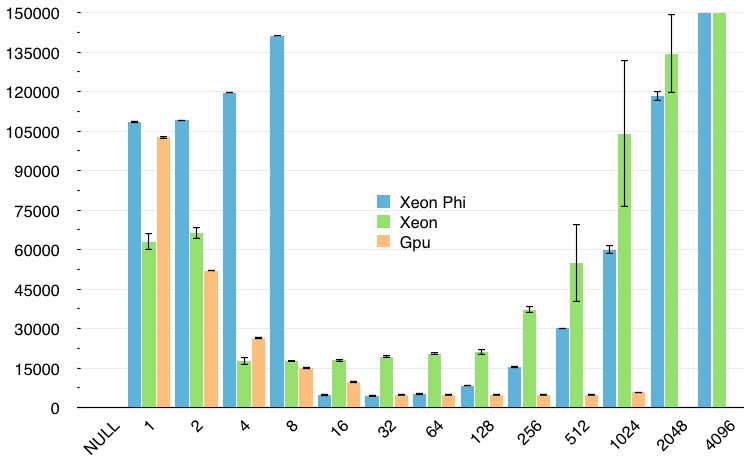
\includegraphics[width=0.6\textwidth]{figures/opt2_comp.png}
    \caption{Row optimisation matrix multiplication with more work in different architectures comparison.}
    \label{RowsComp}
\end{figure}

\begin{figure}[!h]
    \centering
    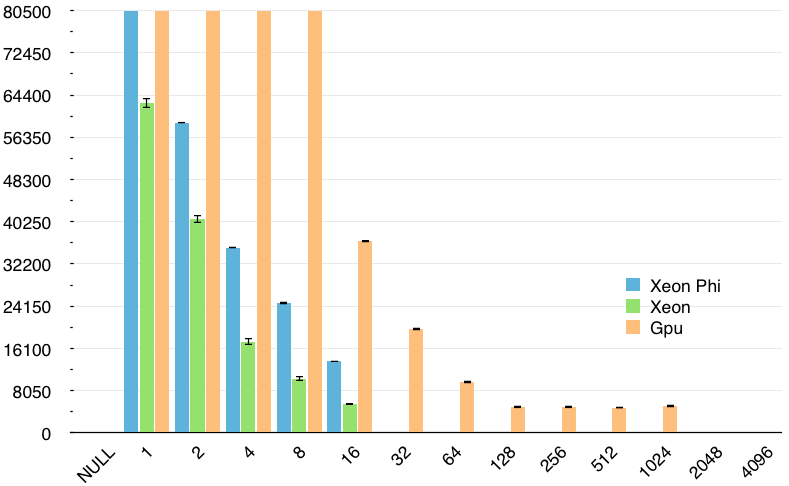
\includegraphics[width=0.6\textwidth]{figures/opt3_comp.png}
    \caption{Rows and columns optimisation matrix multiplication with more work in different architectures comparison.}
    \label{RowsColsComp}
\end{figure}


